\documentclass[letterpaper,10pt,conference]{ieeeconf}
\overrideIEEEmargins

\usepackage{amsmath,amsfonts,amssymb}
\usepackage{graphicx}
\usepackage{cite}
\usepackage{balance}
\usepackage{algorithm, algpseudocode}
\usepackage[bookmarks=true,hidelinks]{hyperref}

\hypersetup{
  pdftitle={Arrodes: Recovering Environmental Beliefs from Ergodic Exploration},
  pdfsubject={Inference of an exploring agent's environmental field belief from observed trajectories},
  pdfkeywords={multi-robot exploration, behavior explanation, world-belief inference, ergodic exploration, empirical orthogonal functions, self-organizing maps},
}

\title{\LARGE \bf
Arrodes: Recovering Environmental Beliefs from Ergodic Exploration
}
\author{Anonymous}

\begin{document}
\maketitle

\begin{abstract}

  In this paper we present a method to address the gap in collaborative exploration that arises when robots cannot share their latest measurements of and beliefs about the environment state. We propose \textit{Arrodes}, an algorithm for inferring the internal world model of an agent exploring an environment through observations of its trajectory. Building off of Bayesian techniques for inferring beliefs in finite, discrete worlds, \textit{Arrodes} uses a self-organizing map (SOM) as a finite, representative space of potential models to perform exact inference when observations are sparse. To handle the limitations of a finite inference space in expressing the potential variability of continuous environmental fields, such as novel transient upwellings in ocean current fields, \textit{Arrodes} also extends to a generalized inference tier using empirical orthogonal functions (EOFs) to capture the continuous space of environment fields. We demonstrate both tiers - finite SOM-based inference and expressive EOF-defined inference - on simulated AUV behavior, using as ground truth a two-year dataset of environment model output around Ram Head on St. John in the U.S. Virgin Islands.

\end{abstract}

\section{Introduction}

Distributed exploration is a multi-robot paradigm for efficiently gathering informative samples of an environment as a group. As robotic agents determine the regions to gather samples from an internal environment model, effective distributed operation relies on the robots' internal models being consistent with one another, and often necessitates communication of measurements and beliefs. Dynamic tasks like monitoring ocean currents pose a two-fold issue to teams, presenting a changing environment that strongly limits communication, resulting in robots soon evolving new beliefs in the world but rendered unable to share their insights \cite{hollinger2012underwater, binney2010informative}. This renders teammates and human supervisors alike with an obfuscated understanding of robot behavior, unable to explain what beliefs, and changes therein, are driving the robot's choices. Without this understanding, team members risk wasting resources covering regions already observed, or worse, not detecting and reacting to novel transient phenomena. This leaves agents with a pressing question: when directly querying models and beliefs that drive a teammate's behavior is infeasible, can observations of its actions reveal in reverse those same beliefs?

\begin{figure}[t]
  \centering
  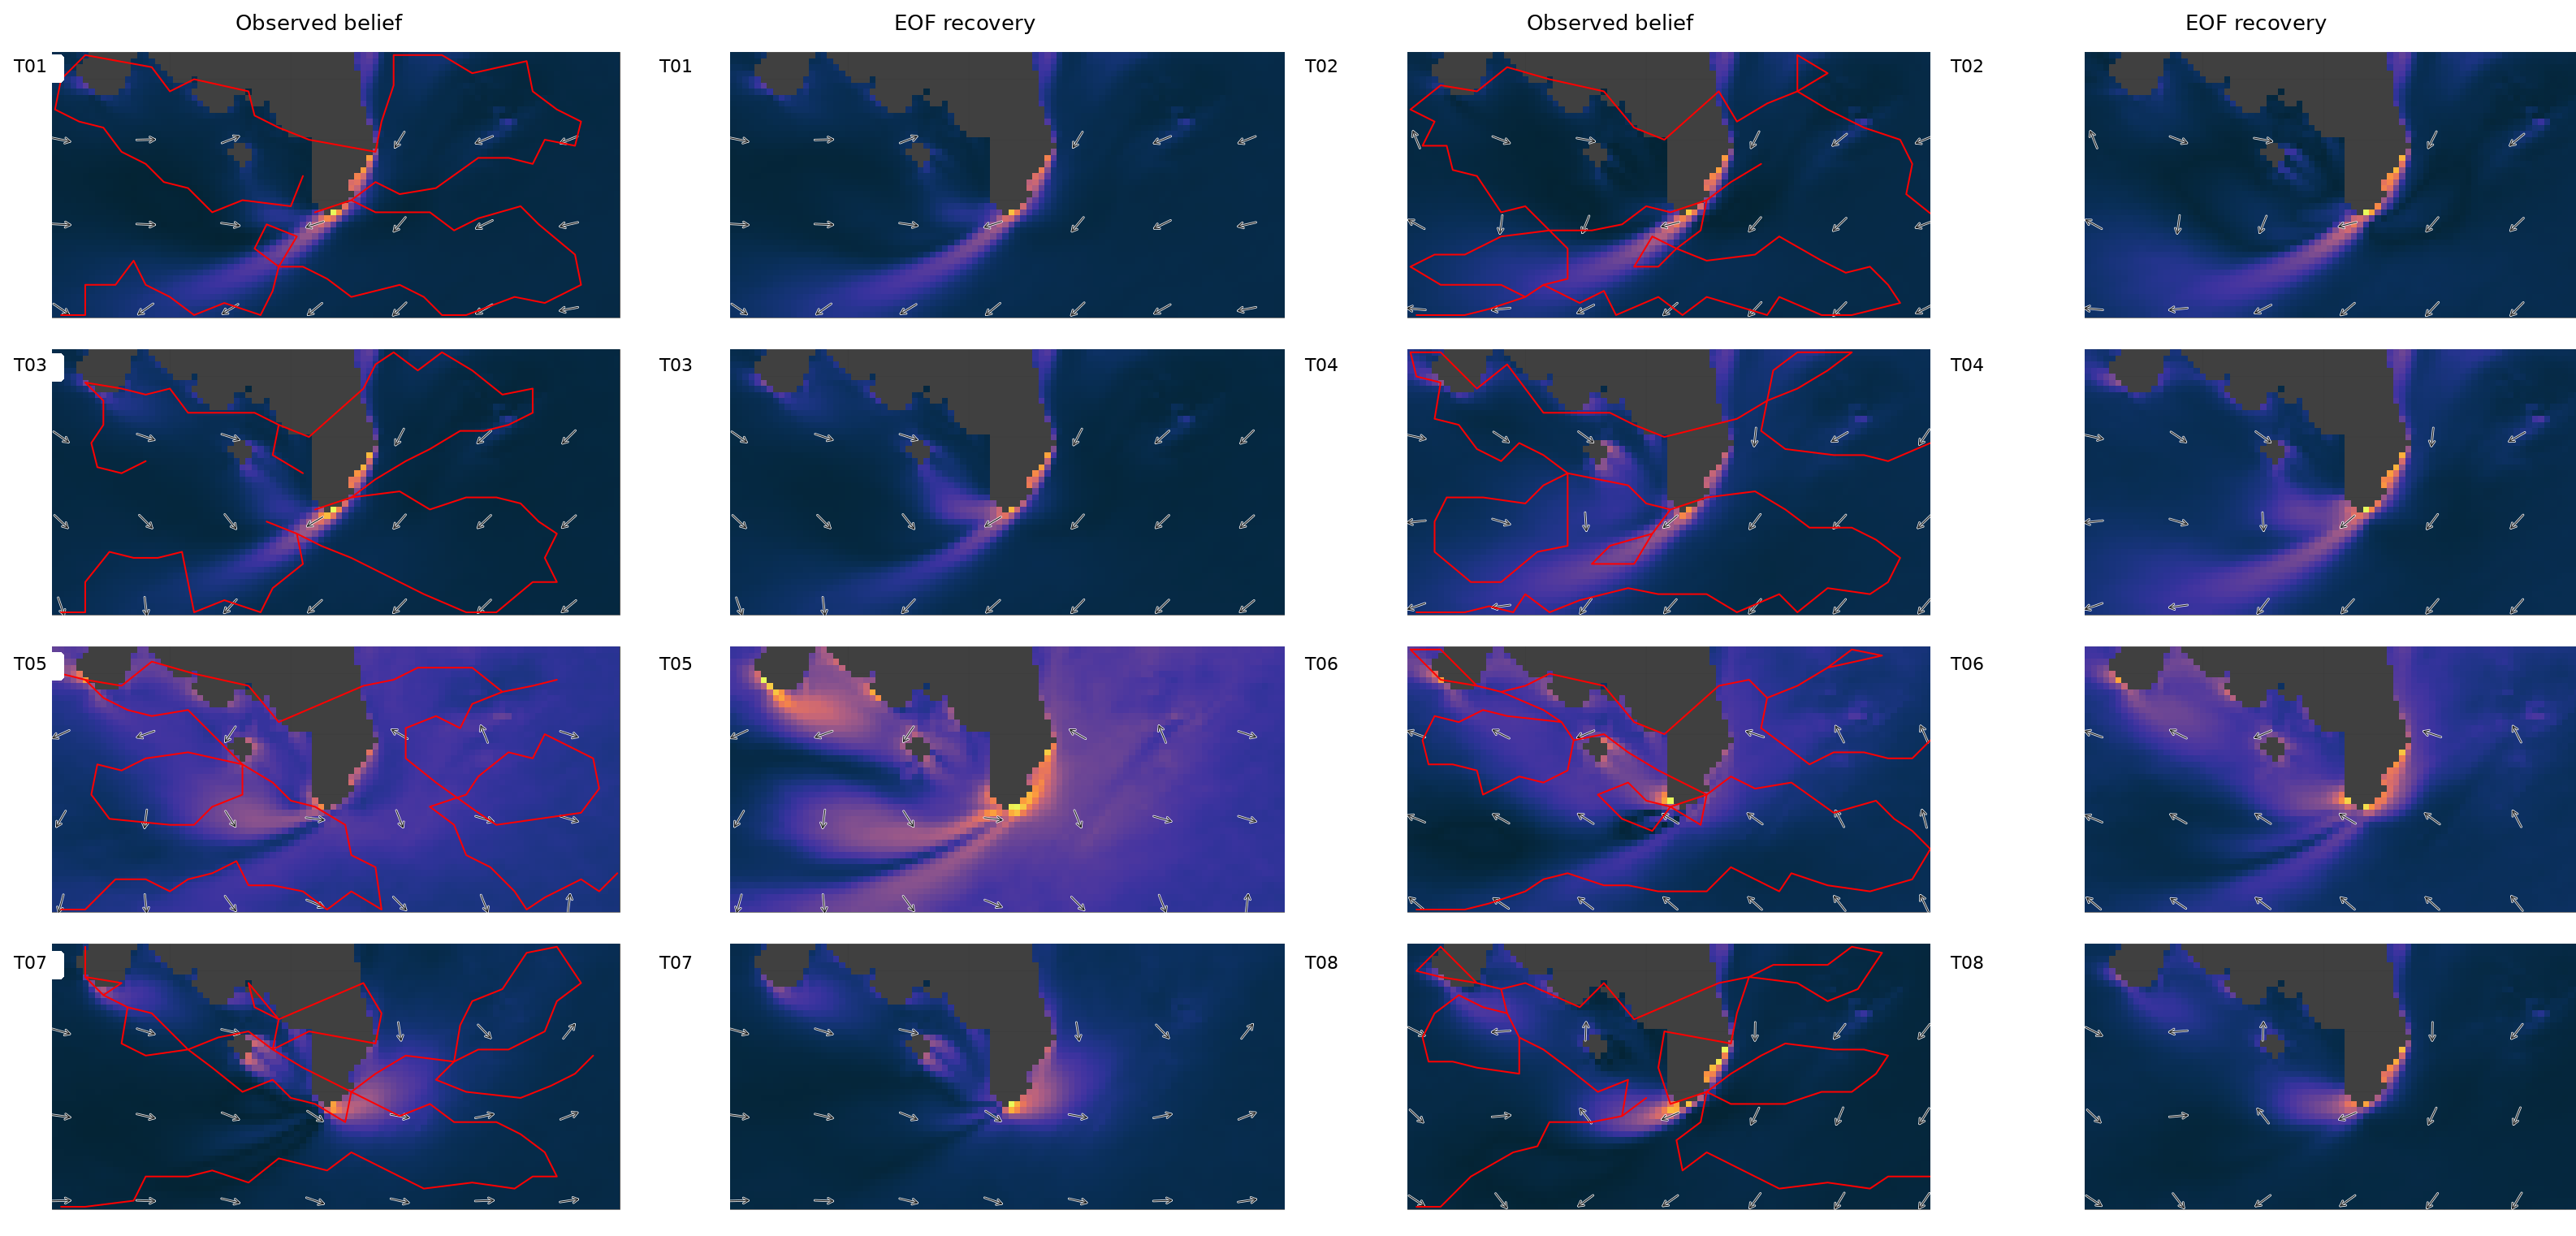
\includegraphics[width=\columnwidth]{figs/front_page_reconstructions.png}
  \caption{Environmental field beliefs inferred from observed motion. Each horizontal pair of plots shows (left) the ground truth environment model of the observed agent, with its observable trajectory in red, followed by (right) Arrodes's reconstruction using the EOF-based inferred posterior. The figures depict the spatial distribution of curl magnitude as a heatmap; arrows show the underlying flow for context.}
  \label{fig:front-reconstructions}
\end{figure}

Belief inference in this manner presents two difficulties. First, exploratory planners determine locations to samples using a transformation of environment belief that helps indicate regions with most promise of interesting information; observers must account for this transformation when reasoning how a sampling route arises from an underlying field. Second, agents are often exploring with respect to continuous fields and gradients, which present a level of variability that finite discretizations of an environment's state struggle to fully characterize, and particularly out-of-distribution novel events. The inference procedure needs a representation of potential environment beliefs that is tractable and sufficiently expressive, and should handle disambiguation from an exploration-centric transformation to the underlying environment model itself.

We address this question through two representations of the environmental models an observed agent might hold. The first adapts Bayesian Theory of Mind (BToM) inference to field exploration: a self-organizing map (SOM) supplies a finite set of complete environmental states, and observed motion provides evidence for each state. Enumeration makes inference exact over this set, although the set itself only approximates the possible beliefs. This distinction matters when a vehicle encounters a structure that its teammates' prior models do not represent.

The second formulation replaces the finite candidate set with continuous coefficients of empirical orthogonal functions (EOFs). The environmental record supplies both spatial modes and a prior over their coefficients. Arrodes uses these quantities for sequential Monte Carlo inference with probabilistic program proposals (SMCP$^{3}$), estimating fields between and beyond the SOM states. This additional capacity comes with an observation requirement: a short route can be consistent with many continuous fields, including fields that explain its current coverage better than the model that generated it.

We present \textit{Arrodes}, an algorithm for inferring an observed agent's environmental field belief from its exploration trajectory. We begin with the Bayesian Theory of Mind formulation of inference over candidate worlds, replacing symbolic alternatives with complete environmental states learned by a self-organizing map (SOM). This allows exact posterior evaluation over a finite set of spatially resolved fields. We then generalize to a continuous space defined by empirical orthogonal functions (EOFs). The EOF basis and a coefficient prior estimated from the environmental record support generative inference using sequential Monte Carlo, allowing reconstruction beyond the fields represented by the SOM.

We focus on ergodic exploration because it relates the spatial distribution of sampling effort to a target derived from the environmental model. Ergodic planning has been demonstrated for underwater sensing \cite{miller2016ergodic} and connects to optimal information gathering under diminishing measurement returns \cite{dressel2018optimality}. This relationship provides a behavioral model for inversion without requiring a particular sequence of actions. It also offers a starting point for inference from other information-gathering planners whose long-horizon sampling exhibits similar spatial statistics.

We evaluate this extension of world-belief inference through simulated flow-field exploration. The trials examine how expanding the space of possible worlds affects reconstruction accuracy and the observations needed for convergence. They also suggest using a sharp decline in ergodic discrepancy as an indicator of when to switch from SOM to EOF inference.

\section{Related Work}

\subsection{Distributed Exploration under Limited Communication}

Informative path planning selects measurements using an agent's current environmental knowledge. In a team, local measurements lead to different models and therefore different sampling decisions. Existing approaches address this dependence through communication scheduling, rendezvous, or explicit reasoning about information available to teammates \cite{binney2010informative,hollinger2012underwater,bramblett2023epistemic}. Arrodes addresses the information needed by such coordination procedures when environmental estimates cannot be exchanged: it infers another vehicle's model from the exploration that model produces.

Reconstructing the model from individual actions is difficult when planning includes stochastic choices and several routes provide comparable information. Ergodic planning supplies a useful alternative description of behavior. It distributes time spent across the domain according to a spatial sampling target \cite{mathew2011ergodicity}, so different routes can be evaluated against the same environmental hypothesis. Miller \emph{et al.}\ demonstrate this approach with underwater electrolocation, including robustness to sensing noise and disturbances \cite{miller2016ergodic}. Subsequent work considers decentralized exploration \cite{abraham2018decentralized}, stochastic sensing dynamics \cite{delatorre2016stochastic}, and motion through time-varying flow fields \cite{hughes2026motionfields}.

Dressel and Kochenderfer identify a class of information-gathering problems for which optimal trajectories are ergodic, under assumptions on diminishing information from repeated measurements \cite{dressel2018optimality}. This connection motivates using spatial sampling statistics to infer environmental belief beyond a particular action sequence. We evaluate that inference with an ergodic planner, as a basis for future extensions to other informative planners.

\subsection{Belief Inference and Behavioral Explanation}

Explaining behavior of autonomous robots often draws from work within cognitive modeling of rational agents and from imitation learning. The latter, commonly leveraged in single- and multi-agent reinforcement learning (MARL) applications, provides an immediate predictor for teammate behavior that is broadly usable across a variety of robotic domains and system representations, and recent work in \cite{garg2021iq, mai2024inverse} avoids the instability in the traditional adversarial learning methods while preserving the breadth of applicability. However, imitation learning aims to arrive at an intermediary layer between internal beliefs and behavior, the policy and Q-function, which serves as a powerful indicator for future actions and interests, but does not truly expose the driving beliefs and motivating factors

Bayesian Theory of Mind explains an agent's actions by reasoning about the beliefs and objectives under which those actions would be expected. Inverse planning has been used to infer goals from approximately rational behavior \cite{baker2009action}, recognize plans \cite{ramirez2010probabilistic}, and account for bounded planning that includes replanning and failed searches \cite{zhixuan2020sips}. These formulations make an agent's internal assumptions explicit, providing explanations that can be evaluated against observed decisions.

Work on belief inference considers further sources of variation in behavior. Interactive POMDP models infer beliefs, preferences, and strategic reasoning \cite{han2018intentional}; inverse decision modeling estimates the decision process \cite{jarrett2021inverse}; and inverse contextual bandits recover evolving knowledge \cite{huyuk2022inverse}. Models of biased world beliefs explain actions that would appear irrational under the observer's knowledge \cite{zhu2026belief}. In cooperative settings, inferred beliefs also support adaptation to partners \cite{muglich2022generalized} and communication about disagreements in plans \cite{zhang2023adaptation}.

Our concern is the representation of the unknown world in this reasoning process. Symbolic planning models describe alternatives through enumerated objects, locations, or facts. This is effective when those alternatives capture the relevant uncertainty, but a continuously varying field requires a different hypothesis space. Moreover, exploratory behavior responds to the sampling value computed from that field, rather than directly to its values. Arrodes retains the Bayesian interpretation of actions as evidence about belief while introducing field representations and a discrepancy model that accounts for this intervening exploration objective.

For scientific autonomy, inferring the environmental model also gives an explanation of a sampling decision. Where general explainability methods identify influential inputs or approximate a controller \cite{angelov2021explainable}, the reconstructed field states what environmental conditions the vehicle's route presumes. Scientists can compare that model with other observations and assess whether the decision serves the mission objective.

\subsection{Representing Possible Environmental Worlds}

McCammon \emph{et al.}\ use SOMs to represent time-varying currents through a finite set of complete flow states learned from historical ocean-model output \cite{mccammon2024som}. Their Bayesian filter updates probabilities over these states from sparse current measurements. The representation retains the spatial resolution of the original fields and can include sharp structures and transitions present in the training record. It offers a practical way to construct the candidate worlds required for belief inference without enumerating combinations of local field values.

Arrodes uses these states as hypotheses about another agent's environmental belief. The evidence is its observed trajectory, evaluated against the sampling target induced by each state. Enumeration gives an exact posterior over the hypotheses, while the reconstructed field remains an approximation limited by the SOM states. An agent that learns about an unfamiliar structure may therefore hold a belief that no mixture of those states adequately represents.

EOFs address this restriction by expressing fields as continuous combinations of spatial modes. We use the environmental representation under development in SCRIBE \cite{scribe2026}: the prior record supplies a mean field, a basis, and a coefficient covariance. These quantities define both a continuous hypothesis space and a prior for proposing candidate fields. Arrodes performs inference in that space using SMCP$^3$ \cite{lew2023smcp3}, whose paired proposals support structured particle updates. The resulting generalization preserves inference over explicit world models while allowing combinations unavailable to the finite SOM representation.

\section{Problem Formulation and Environmental Models}

\subsection{Problem Statement}

Let $\mathcal X$ be the spatial domain and let $f^\star\in\mathcal F$ be the static environmental field estimate guiding an observed agent. An ego agent receives a sequence
\begin{equation}
  z_{1:T}=\{(x_q,d_q)\}_{q=1}^{T}
\end{equation}
of visited locations $x_q\in\mathcal X$ and dwell times $d_q$. It knows the exploration objective $r:\mathcal F\times\mathcal X\rightarrow\mathbb R_{\geq0}$ and assumes that the observed agent allocates coverage ergodically with respect to the resulting sampling target. It does not receive the measurements from which $f^\star$ was formed. We call $f^\star$ the \emph{generating field} and $z_{1:t}$ the \emph{observed trajectory prefix}.

The objective assigns sampling value $r(f,x)$ to location $x$ under a candidate field $f$. At quadrature locations $\xi_1,\ldots,\xi_M$ with spatial weights $w_m$, it induces the probability masses
\begin{equation}
  \mu_m(f)=\frac{w_m r(f,\xi_m)}{\sum_{j=1}^{M}w_jr(f,\xi_j)}.
  \label{eq:target-measure}
\end{equation}
We call $\mu(f)$ the \emph{sampling target}. Arrodes infers
\begin{equation}
  p_t(f)=p(f\mid z_{1:t},r),\quad
  \widehat f_t=\mathbb E_{p_t}[f],\quad
  \widehat\mu_t=\mathbb E_{p_t}[\mu(f)].
  \label{eq:inference-problem}
\end{equation}
The posterior mean $\widehat f_t$ is the reconstructed field shown in Fig.~\ref{fig:front-reconstructions}; $\widehat\mu_t$ describes the corresponding posterior expectation over sampling targets. Fields that induce similar sampling targets may remain difficult to distinguish, and the posterior retains this ambiguity.

Here $f^\star$ is the observed agent's estimate, which may differ from the physical environment. The ego agent's posterior describes uncertainty about that estimate, not a direct update from ocean measurements. Holding the exploration objective fixed separates this problem from goal inference: disagreement between the recovered field and the ego agent's own field can explain different sampling decisions even when both agents pursue the same scientific task.

\subsection{Inference from Exploration}

For each candidate field, Arrodes computes a sampling target using the known objective and compares it with the observed trajectory's spatial distribution. This discrepancy determines a posterior over SOM states or EOF coefficients, from which the field is reconstructed by posterior averaging. Algorithm~\ref{alg:arrodes} summarizes the computation; Sec.~IV defines the discrepancy and posterior updates.

\begin{algorithm}[H]
\caption{Arrodes environmental belief inference}
\label{alg:arrodes}
\footnotesize
\begin{algorithmic}[1]
\Require trajectory $z_{1:T}$, objective $r$, SOM states $\{s_k,\rho_k\}$
\Require EOF model $(\bar f,\Phi,p_0)$ and behavioral score parameters
\State Compute the sampling target $\mu(s_k)$ for every SOM state
\State Draw EOF coefficient particles $\boldsymbol a^{1:N}\sim p_0$
\For{$t=1,\ldots,T$}
  \State Form the occupation measure of $z_{1:t}$
  \State Evaluate $D_t(s_k)$ and normalize the finite SOM posterior
  \State Evaluate $D_t(f_{\boldsymbol a})$ and update the EOF particle posterior
  \State Resample and rejuvenate the EOF particles when required
  \State Reconstruct $\widehat f_t^{\mathrm{SOM}}$ and $\widehat f_t^{\mathrm{EOF}}$
\EndFor
\State \Return both posterior histories and reconstructed fields
\end{algorithmic}
\end{algorithm}

\subsection{Finite SOM Model}

A SOM organizes learned environmental states on a graph $\mathcal G=(V,E_G)$. During training, the closest prototype and its graph neighbors move toward each sampled environmental state \cite{mccammon2024som}. Each learned state defines a field $s_k\in\mathbb R^G$ in the representation used for inference, where $G$ is the number of spatial field values. The resulting family retains recurring environmental patterns and the neighborhood relationships among them. Arrodes uses
\begin{equation}
  \mathcal F_{\mathrm{SOM}}=\{s_1,\ldots,s_K\}
  \label{eq:som-worlds}
\end{equation}
as its finite hypotheses. A posterior over the vertices identifies learned states consistent with the trajectory, while the posterior mean $\sum_k p_t(k)s_k$ reconstructs a mixture of those states.

\subsection{Continuous EOF Model}

The continuous model uses an EOF expansion within the environmental modeling approach being developed in SCRIBE \cite{scribe2026}. Let $f^{(1)},\ldots,f^{(H)}\in\mathbb R^G$ be fields from the prior environmental record, $\bar f$ their mean, $W=\operatorname{diag}(v_1,\ldots,v_G)$ the full-field spatial weight matrix, and
\begin{equation}
  \bar f=\frac{1}{H}\sum_{h=1}^{H}f^{(h)},\quad
  X=\left[f^{(1)}-\bar f,\ldots,f^{(H)}-\bar f\right].
\end{equation}
From the weighted singular value decomposition
\begin{equation}
  W^{1/2}X=U\Sigma V^\top,
\end{equation}
we retain $R$ modes and set $\Phi=W^{-1/2}U_{:,1:R}$. The weighted orthogonality $\Phi^\top W\Phi=I_R$ gives the projection and reconstruction
\begin{equation}
  \boldsymbol a(f)=\Phi^\top W(f-\bar f),\qquad
  f_{\boldsymbol a}=\bar f+\Phi\boldsymbol a.
  \label{eq:eof-field}
\end{equation}
The ego agent supplies the Gaussian prior $p_0(\boldsymbol a)=\mathcal N(\boldsymbol a;\boldsymbol a_0,P_0)$. In the simulated trials, $\boldsymbol a_0=\boldsymbol0$ reconstructs the mean environment and $P_0$ retains the correlated coefficient variation estimated from the prior record. Projecting each SOM state through \eqref{eq:eof-field} places the finite hypotheses and continuous particles in the same rank-$R$ coefficient geometry. The SOM posterior still reconstructs its complete prototype fields; the coefficient projection is used to compare their environmental support with that of the continuous model.

\section{Behavior-Conditioned Inference}

\subsection{Trajectory Discrepancy and Behavioral Evidence}

The occupation measure of the observed trajectory prefix is
\begin{equation}
  \nu_t=\sum_{q=1}^{t}\omega_q\delta_{x_q},\qquad
  \omega_q=\frac{d_q}{\sum_{j=1}^{t}d_j}.
  \label{eq:occupation}
\end{equation}
An ergodic planner drives this measure toward its sampling target. We evaluate a candidate field with the squared maximum mean discrepancy
\begin{equation}
  D_t(f)=\operatorname{MMD}_k^2\!\left(\nu_t,\mu(f)\right).
  \label{eq:mmd}
\end{equation}
For the Gaussian kernel $k_\ell(x,y)=\exp[-\|x-y\|^2/(2\ell^2)]$, the discrepancy has the explicit form \cite{gretton2012mmd}
\begin{equation}
\begin{split}
 D_t(f)={}&\sum_{q,s=1}^{t}\omega_q\omega_s k_\ell(x_q,x_s)\\
 &-2\sum_{q=1}^{t}\sum_{m=1}^{M}\omega_q\mu_m(f)k_\ell(x_q,\xi_m)\\
 &+\sum_{m,n=1}^{M}\mu_m(f)\mu_n(f)k_\ell(\xi_m,\xi_n).
\end{split}
\label{eq:mmd-expanded}
\end{equation}
The first term describes the observed coverage, the last describes the candidate target, and the cross term measures their spatial agreement. Nearby visits contribute through their kernel similarity, avoiding a hard partition into spatial bins. The discrepancy therefore expresses the assumed allocation relationship without assigning an independent likelihood to each control action.

A short prefix has covered only part of its target and should exert less influence than a mature trajectory. Arrodes uses the behavioral energy and generalized likelihood
\begin{equation}
  \mathcal E_t(f)=\frac{\beta_t}{s_D}D_t(f),\qquad
  L_t(f)=\exp[-\mathcal E_t(f)],
  \label{eq:energy}
\end{equation}
with
\begin{equation}
  \beta_t=\beta_{\max}\frac{t^p}{t^p+t_{1/2}^{p}}.
  \label{eq:maturity}
\end{equation}
The scale $s_D$ is the median pairwise target-measure discrepancy, calibrated using prior environmental fields for EOF inference and learned states for SOM inference. At observation $t$, the likelihood is evaluated against the complete prefix $z_{1:t}$; successive cumulative prefixes are not treated as independent trajectories.

\subsection{Finite SOM Update}

Let $\rho_k$ be the prior probability of SOM state $s_k$. Since the hypothesis set is finite, Arrodes evaluates its posterior directly:
\begin{equation}
  p_t(k)=\frac{\rho_k L_t(s_k)}{\sum_{j=1}^{K}\rho_jL_t(s_j)},\qquad
  \widehat f_t^{\mathrm{SOM}}=\sum_{k=1}^{K}p_t(k)s_k.
  \label{eq:som-posterior}
\end{equation}
This update is exact within the finite model. To align the initial preference of both formulations, the SOM states are projected to EOF coefficients $\boldsymbol a_k$ and assigned
\begin{equation}
  \rho_k\propto\exp\!\left[-\tfrac12(\boldsymbol a_k-\boldsymbol a_0)^\top
  P_0^{-1}(\boldsymbol a_k-\boldsymbol a_0)\right].
  \label{eq:som-prior}
\end{equation}
The posterior can quickly concentrate on complete learned states, but every reconstructed field remains a mixture of the SOM prototypes.

\subsection{Continuous EOF Update}

The EOF formulation conditions the Gaussian coefficient prior on the same behavioral evidence,
\begin{equation}
  \pi_t(\boldsymbol a)\propto p_0(\boldsymbol a)
  \exp[-\mathcal E_t(f_{\boldsymbol a})].
  \label{eq:eof-posterior}
\end{equation}
This posterior can occupy coefficient combinations absent from the finite model, while remaining limited by the retained EOF basis. Arrodes represents \eqref{eq:eof-posterior} in Gen \cite{cusumano2019gen} and uses paired forward and backward proposals to move particles between successive prefix-conditioned targets, following SMCP$^3$ \cite{lew2023smcp3}.

The proposal follows a local Gauss--Newton approximation. Let $m_t$ be the locally optimized coefficient vector, $J_t=\partial\mu(f_{\boldsymbol a})/\partial\boldsymbol a|_{m_t}$, and $\mathbf K$ the spatial kernel matrix at the quadrature sites. The transport covariance is
\begin{equation}
  C_t=\gamma\left(P_0^{-1}+\frac{2\beta_t}{s_D}J_t^\top \mathbf KJ_t\right)^{-1},
  \qquad C_t=B_tB_t^\top,
  \label{eq:proposal-covariance}
\end{equation}
where $\gamma$ scales the covariance. Consecutive approximations define the affine map
\begin{equation}
  T_t(\boldsymbol a)=m_t+B_tB_{t-1}^{-1}(\boldsymbol a-m_{t-1}).
  \label{eq:transport}
\end{equation}
The backward proposal applies $T_t^{-1}$. Writing $\widetilde\pi_t=p_0L_t$ for the unnormalized target, a transported particle $\boldsymbol a_t^i=T_t(\boldsymbol a_{t-1}^i)$ receives weight
\begin{equation}
 \widetilde w_t^i=w_{t-1}^i
 \frac{\widetilde\pi_t(\boldsymbol a_t^i)}
      {\widetilde\pi_{t-1}(\boldsymbol a_{t-1}^i)}
 \left|\det(B_tB_{t-1}^{-1})\right|.
 \label{eq:transport-weight}
\end{equation}
Normalizing these weights corrects both the change in behavioral evidence and the volume change under transport. Thus the local Gaussian approximation guides particle motion while the weights continue to target \eqref{eq:eof-posterior}. In particular, a short prefix may move the local approximation toward a field explaining only the portion of the domain visited so far.

When $N_{\mathrm{eff}}=(\sum_i(w_t^i)^2)^{-1}$ falls below a fraction of the particle count, residual resampling allocates copies according to the weights. Metropolis--Hastings moves then propose coefficient alternatives and accept them using the posterior and proposal-density ratio. These moves preserve $\pi_t$ while allowing replicated particles to explore distinct explanations. The environmental reconstruction is
\begin{equation}
 \widehat f_t^{\mathrm{EOF}}=\bar f+\Phi\sum_{i=1}^{N}w_t^i\boldsymbol a_t^i.
\end{equation}
Continuous inference incurs greater computation than finite enumeration, but supports recovery between and beyond the learned SOM states.

\section{Simulated Ocean Exploration}

\subsection{Environmental Record and Mission}

We use two years of hourly surface-current output from a Regional Ocean Modeling System hindcast of an approximately $2\,\mathrm{km}^2$ coastal region west of Ram Head, St. John, U.S. Virgin Islands \cite{shchepetkin2005roms,mccammon2024som}. Retaining every third snapshot gives 5,680 environmental states. To focus sampling on rotational flow structures, each state is represented by the magnitude of vertical curl divided by its spatial mean. The first 80\% of the time-ordered record determines a rank-10 EOF model. The next 568 states calibrate the coefficient covariance and discrepancy scale; the final 568 provide candidate generating fields. A $7\times7$ SOM trained on the velocity history supplies 49 finite states, with each velocity prototype transformed into the same curl-shape representation.

For a field $f$, the simulated objective uses $r(f,x)=|f(x)|+\epsilon$, with $\epsilon$ equal to $0.01$ times the training-field standard deviation. The field values remain in their unit-mean curl-shape representation for reconstruction and RMSE. Only the quadrature masses in \eqref{eq:target-measure} are normalized for trajectory planning and discrepancy evaluation.

The ego prior is centered at $\boldsymbol a_0=\boldsymbol0$, the EOF mean environment, with the correlated covariance estimated from the calibration record. Both formulations use 196 quadrature sites and a Gaussian kernel bandwidth of $0.2$ in normalized domain coordinates. For every generating field, the observed agent follows a 100-location kernel-ergodic trajectory toward its sampling target. Arrodes receives those locations and their dwell times, but none of the environmental data available to the observed agent. Continuous inference uses 512 particles, an effective-sample-size threshold of $0.65N$, two rejuvenation steps, and $\beta_{\max}=125$, $t_{1/2}=18$, and $p=2$. The proposal uses eight local optimization steps and $\gamma=1$. The planner uses 180 optimization iterations, unit dwell weights, and a speed of $0.0625$ in domain coordinates per second; temporal plots use cumulative path length divided by this speed.

\subsection{Distance from the Finite Representation}

The role of continuous inference becomes clearest as the generating field leaves the region available to the SOM posterior mean. Let $P_0=B_0B_0^\top$ and define prior-whitened coefficients
\begin{equation}
  \boldsymbol y(\boldsymbol a)=B_0^{-1}(\boldsymbol a-\boldsymbol a_0).
\end{equation}
For projected SOM coefficients $\boldsymbol a_1,\ldots,\boldsymbol a_K$, let $Y=[\boldsymbol y(\boldsymbol a_1),\ldots,\boldsymbol y(\boldsymbol a_K)]$. The coefficient region available to every posterior-weighted SOM reconstruction is the convex hull
\begin{equation}
  \mathcal H_{\mathrm{SOM}}=\{Y\boldsymbol\lambda:\boldsymbol\lambda\geq0,
  \ \boldsymbol1^\top\boldsymbol\lambda=1\}.
\end{equation}
We measure a generating field's departure from this region by
\begin{equation}
  \delta_{\mathrm{SOM}}(\boldsymbol a)=
  \min_{\boldsymbol\lambda\in\Delta_K}
  \|\boldsymbol y(\boldsymbol a)-Y\boldsymbol\lambda\|_2.
  \label{eq:som-distance}
\end{equation}
One unit of $\delta_{\mathrm{SOM}}$ is one standard deviation in the correlated EOF prior geometry.

We compute \eqref{eq:som-distance} offline for all 568 candidate fields, then select five temporally separated fields near each of ten distances across the available range. Two planner starting positions generate different observable trajectories from every field, yielding 100 simulated trials. The group-mean distances range from $0.61$ to $4.78$ prior standard deviations. We report spatially weighted field RMSE; aggregate markers show the mean across ten trajectories at each distance and error bars show one standard deviation.

\begin{figure*}[t]
  \centering
  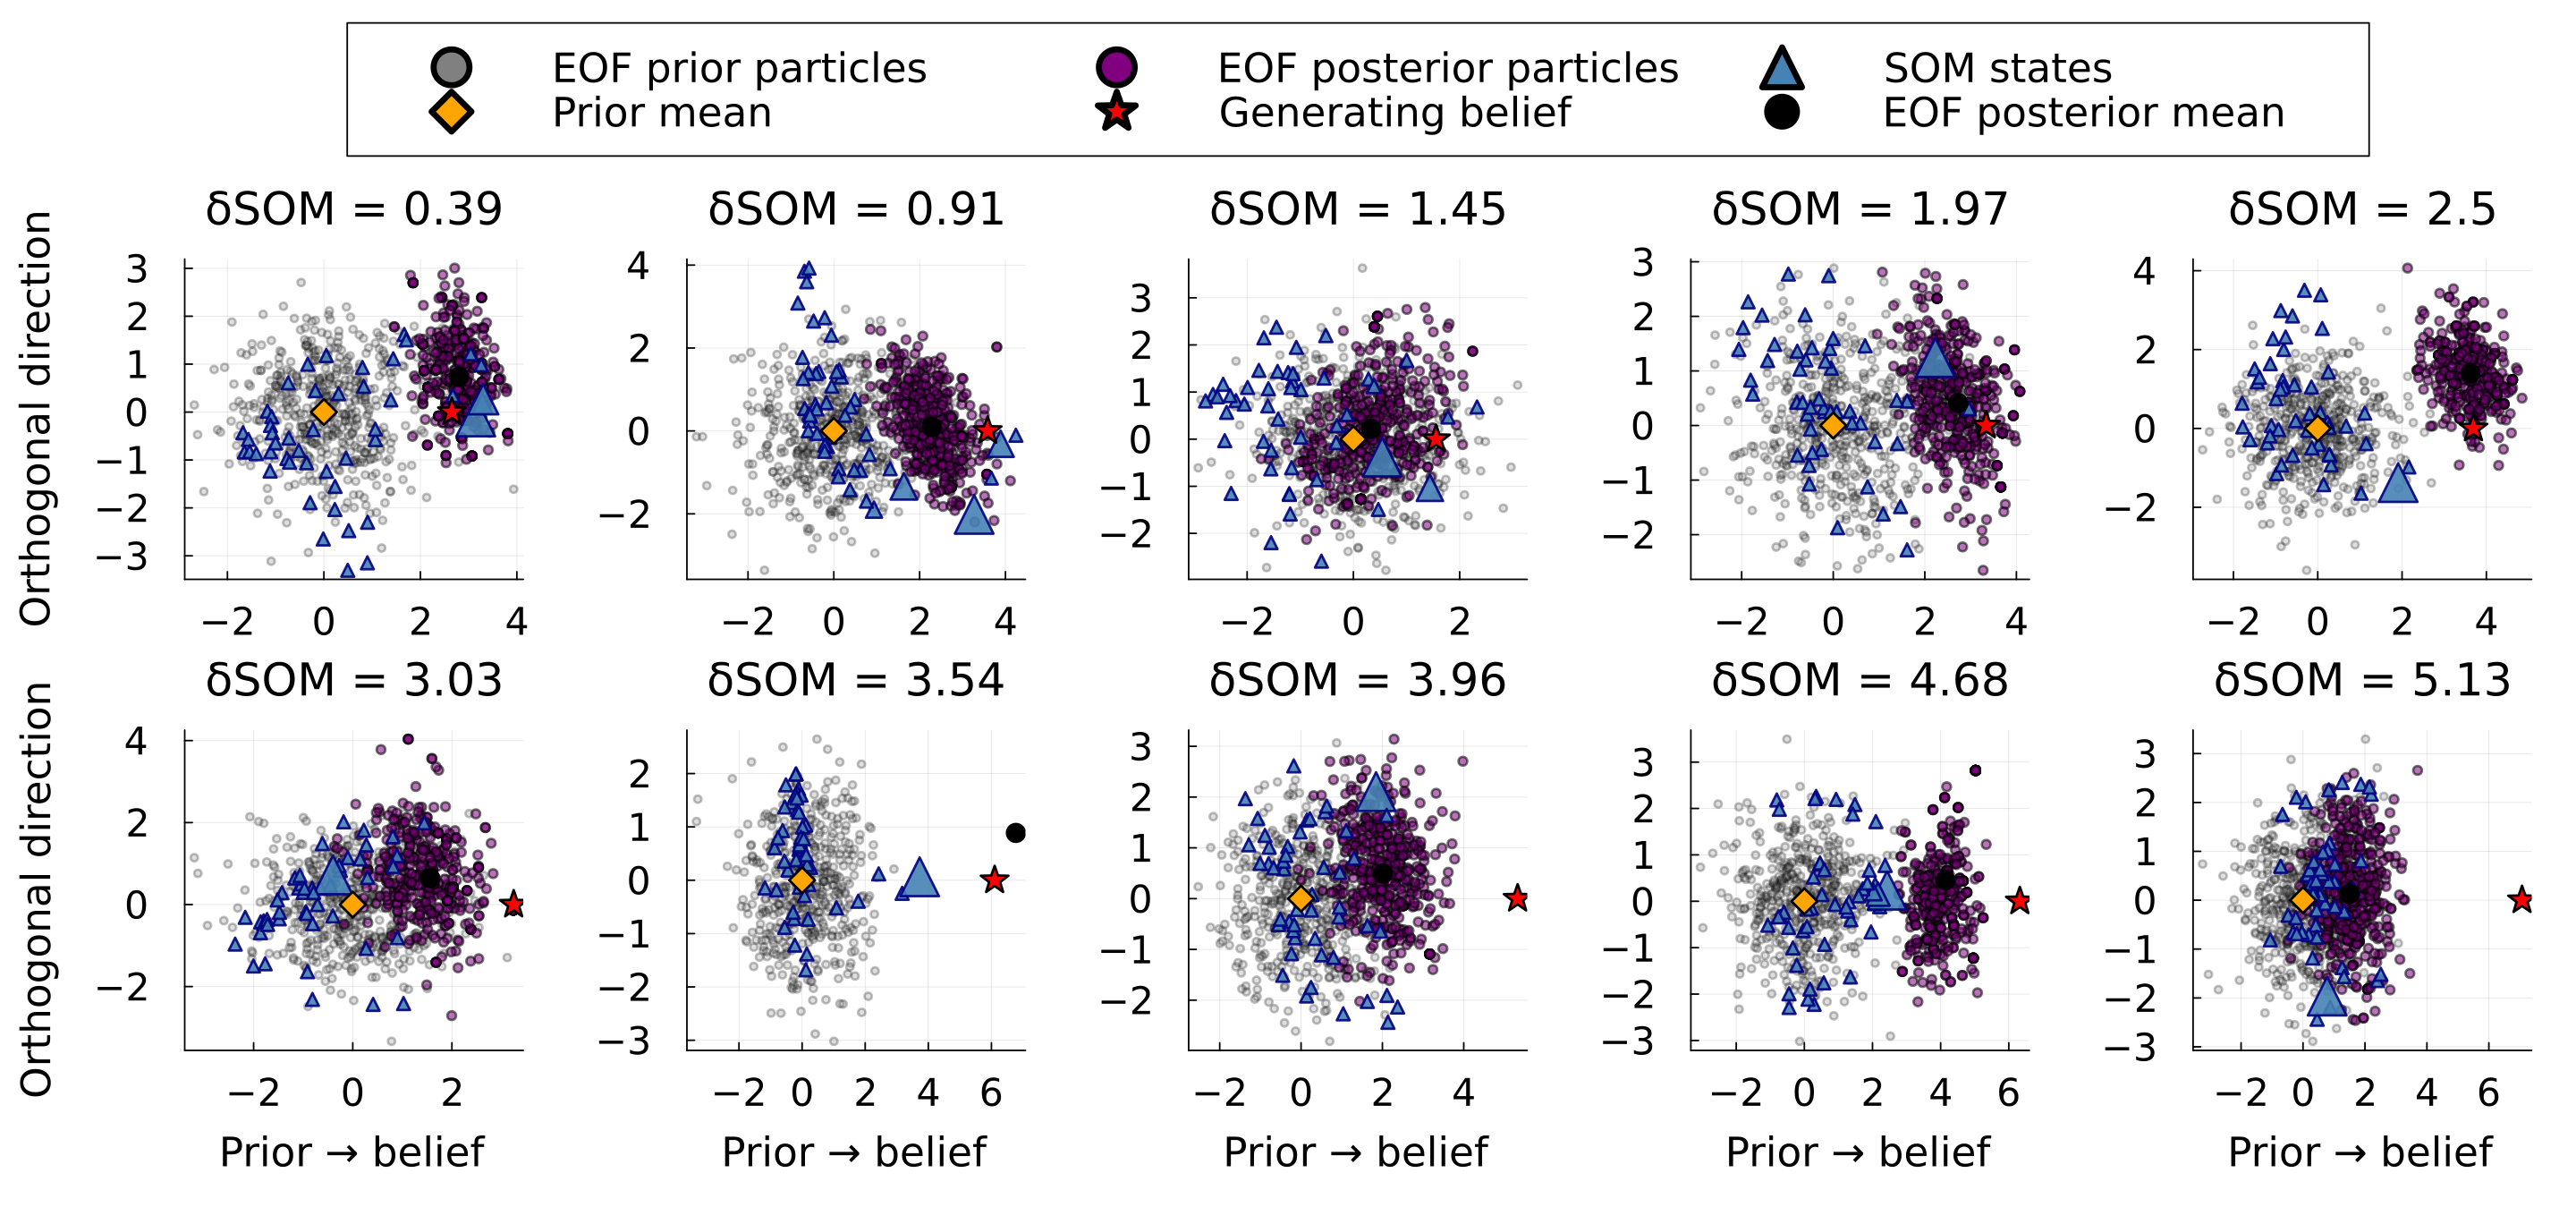
\includegraphics[width=0.96\textwidth]{figs/all_world_space_trials.png}
  \caption{The finite and continuous beliefs occupy the same EOF coefficient space. Across fields at increasing distance $\delta_{\mathrm{SOM}}$ from the SOM region, the continuous particles move from the mean-environment prior toward fields whose sampling targets explain the observed trajectory. The SOM states delimit the region available to the finite posterior mean; each panel projects onto the direction from the prior mean to the generating belief and an orthogonal direction of posterior variation. Coordinates are in prior standard deviations; distances are evaluated in the full coefficient space. Triangle size indicates SOM posterior support.}
  \label{fig:world-space}
\end{figure*}

\section{Results}

\subsection{Reconstructing the Observed World Belief}

The inferred fields in Fig.~\ref{fig:front-reconstructions} recover prominent circulation structures in the observed agent's belief from its trajectory alone. Their location and extent explain the agent's concentration of sampling effort. Fine structure is less completely recovered, but the reconstructions distinguish different environmental beliefs without access to the measurements that produced them.

Figure~\ref{fig:world-space} shows how these reconstructions depart from the ego agent's prior. The EOF posterior particles move away from the mean-environment prior toward the generating belief, while the SOM posterior selects among existing states. Their common coefficient coordinates show the extension afforded by EOF inference: reconstructed fields can lie beyond the region spanned by SOM mixtures.

\subsection{Recovery beyond the SOM Region}

\begin{figure}[t]
  \centering
  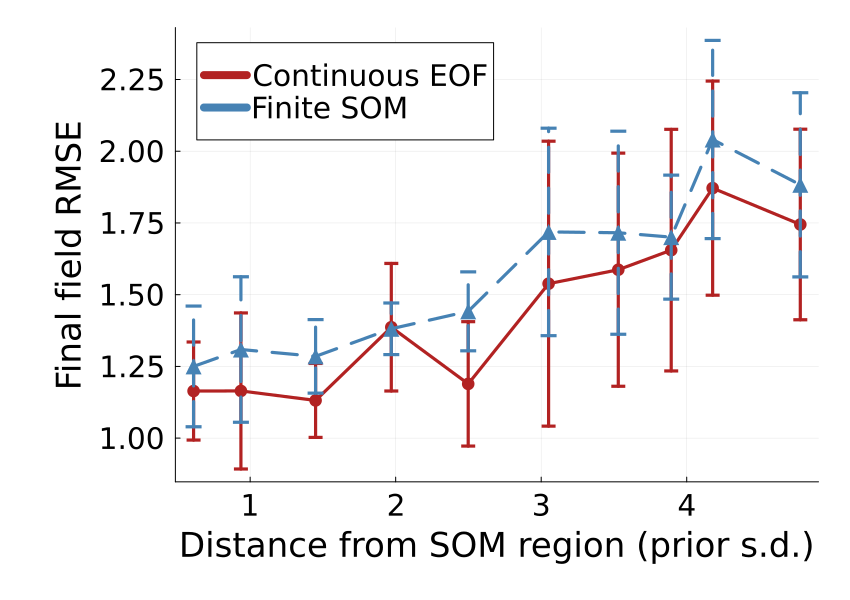
\includegraphics[width=\columnwidth]{figs/final_recovery_by_som_distance.png}
  \caption{Final field recovery as the generating field moves away from the region spanned by the SOM states. Markers show mean reconstruction error over repeated fields and starting positions at their actual mean distance; error bars show one standard deviation. EOF inference generally yields a closer reconstruction, with substantial variation across fields and starting positions.}
  \label{fig:final-recovery}
\end{figure}

The SOM reconstruction remains a useful approximation, but its error increases as generating fields depart from the learned states. The EOF formulation can account for some of this departure by adjusting coefficients beyond the SOM region.

EOF inference achieves lower mean final RMSE at nine of the ten distances in Fig.~\ref{fig:final-recovery}; the SOM mean is marginally lower near $\delta_{\mathrm{SOM}}=1.97$. Variation across generating fields and starting positions is substantial, so this is an overall improvement rather than uniform dominance. The expanded representation permits closer recovery of beliefs that the SOM can only approximate.

\subsection{Trajectory Coverage Governs Continuous Recovery}

This improvement requires a longer observation history. In Fig.~\ref{fig:detailed-recovery}, EOF field error initially rises while even the generating target has high discrepancy with the observed trajectory. Fields matching the incomplete route can therefore receive more support than the belief that actually generated it. As the route covers more of the target, discrepancy falls and both field and target reconstruction improve.

\begin{figure*}[p]
  \centering
  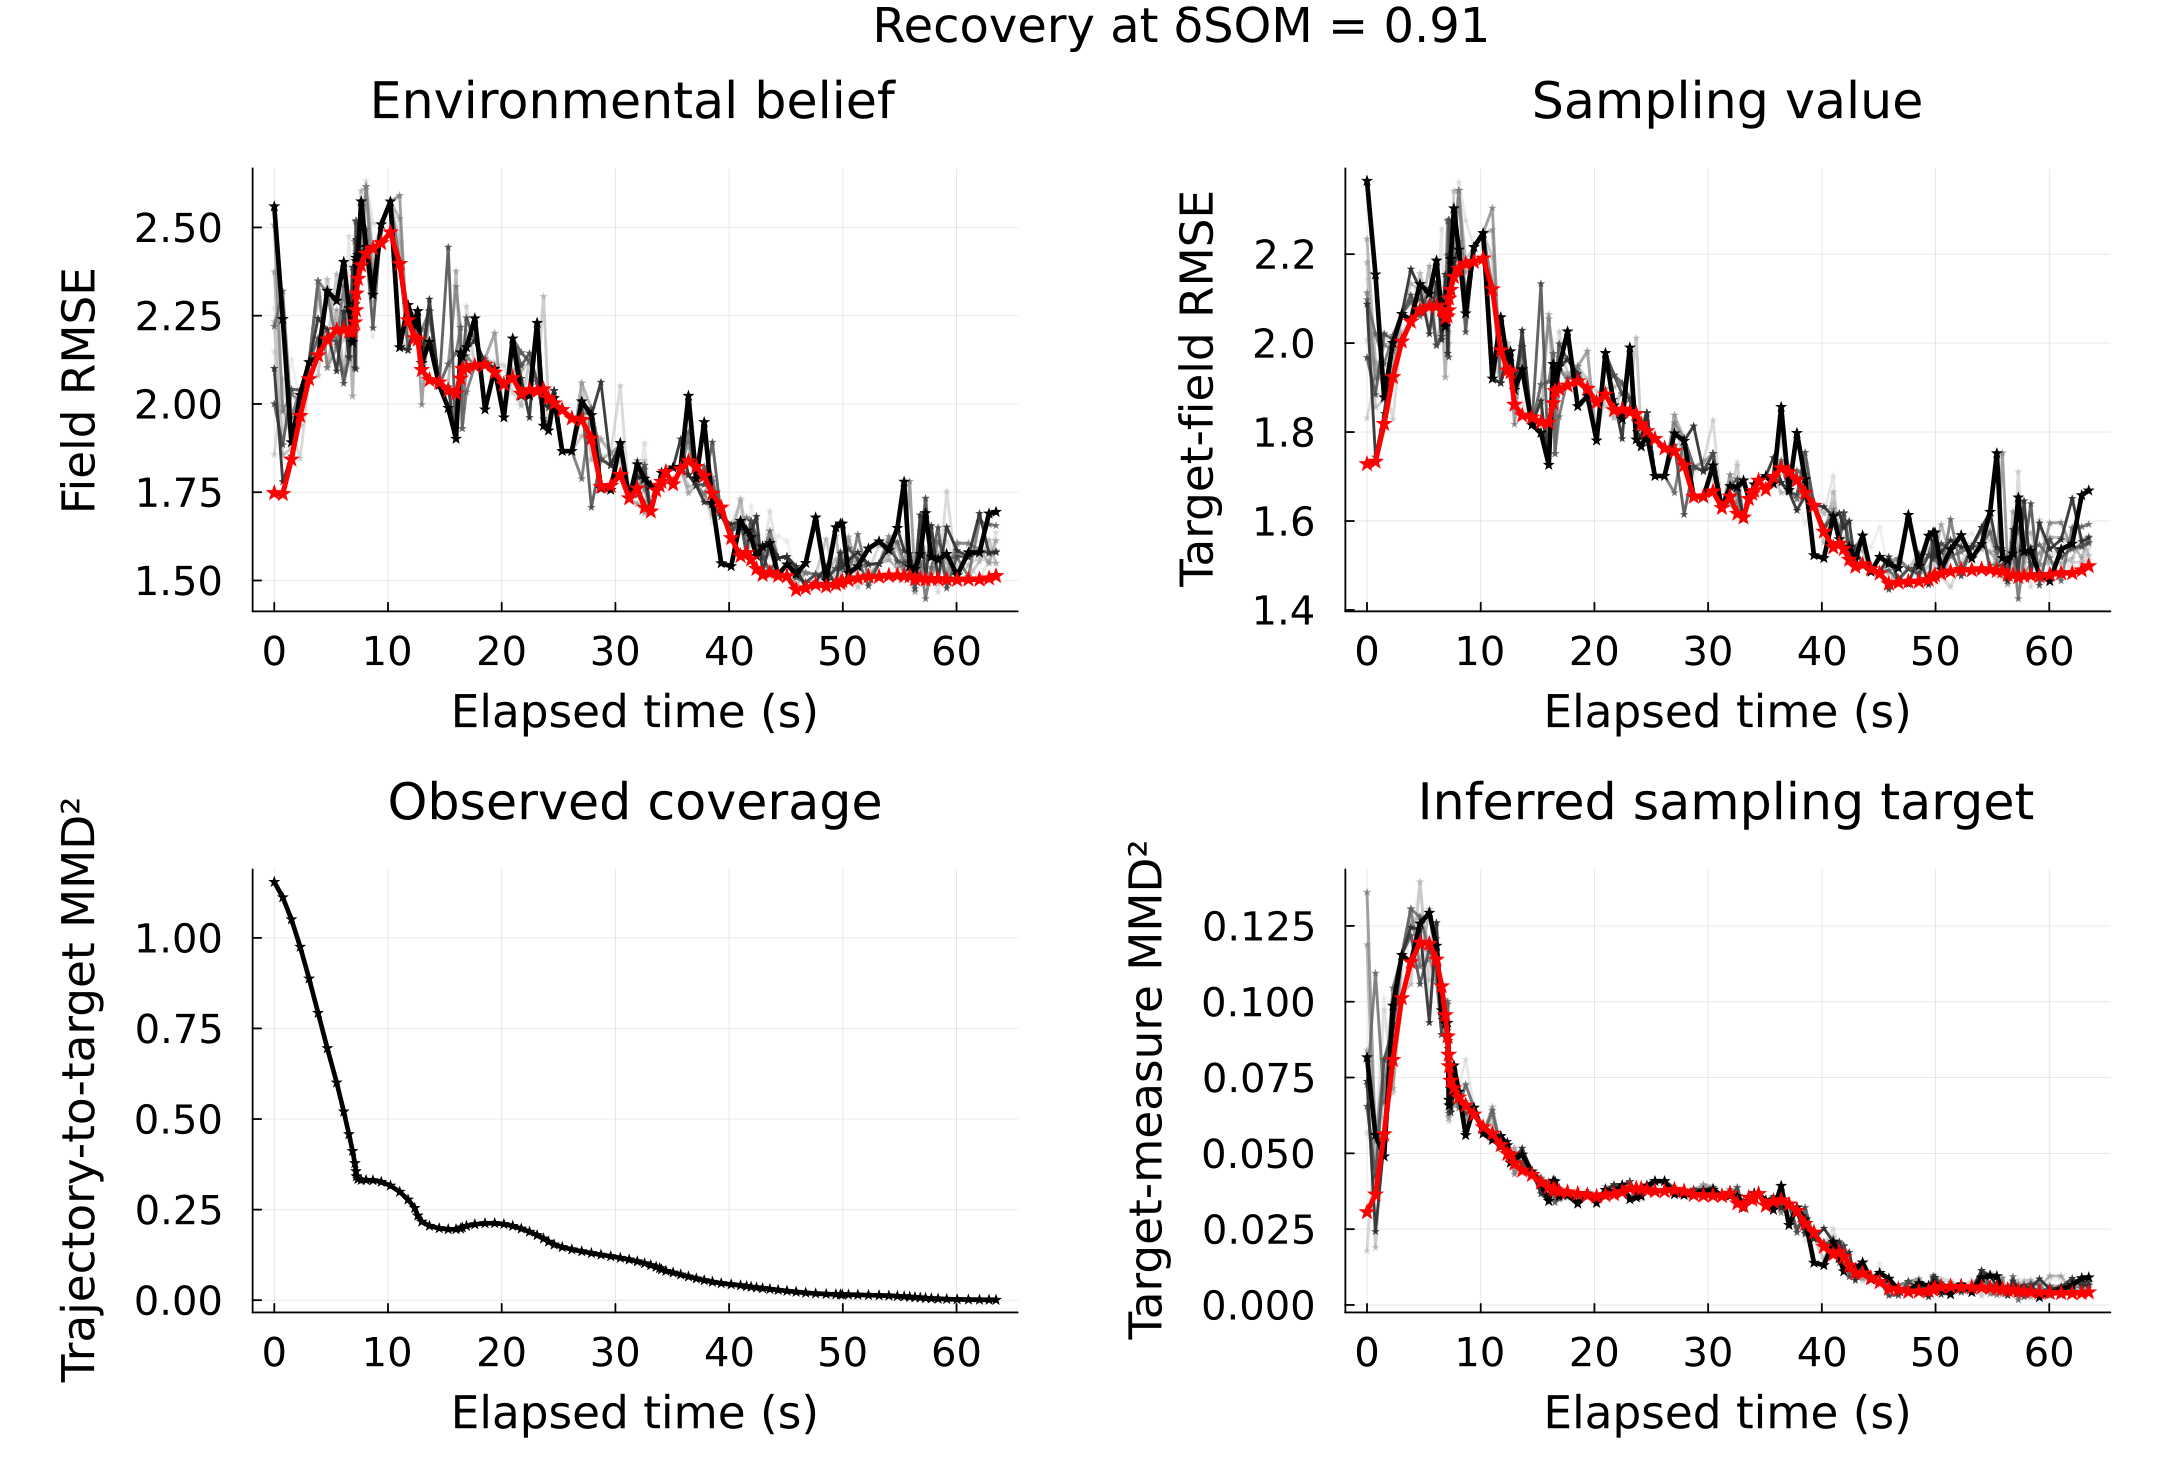
\includegraphics[width=0.88\textwidth]{figs/detailed_recovery_trial_02.png}
  \caption{Continuous reconstruction develops as coverage becomes representative, shown near the SOM region ($\delta_{\mathrm{SOM}}=0.91$). The upper panels show environmental-field and target-field RMSE; gray curves describe highly weighted particles and red curves their posterior aggregate. The lower left shows trajectory-to-generating-target MMD$^2$; the lower right shows inferred-target discrepancy relative to the EOF representation of the generating belief. The early rise and subsequent decline in reconstruction error occur as the trajectory becomes more representative of its generating target.}
  \label{fig:detailed-recovery}
\end{figure*}

The histories in Fig.~\ref{fig:recovery-histories} show this behavior across the range of distances. SOM estimates often settle early, while EOF estimates undergo transient error increases before improving. The additional observations constrain continuous alternatives that a short route cannot distinguish.

\begin{figure*}[p]
  \centering
  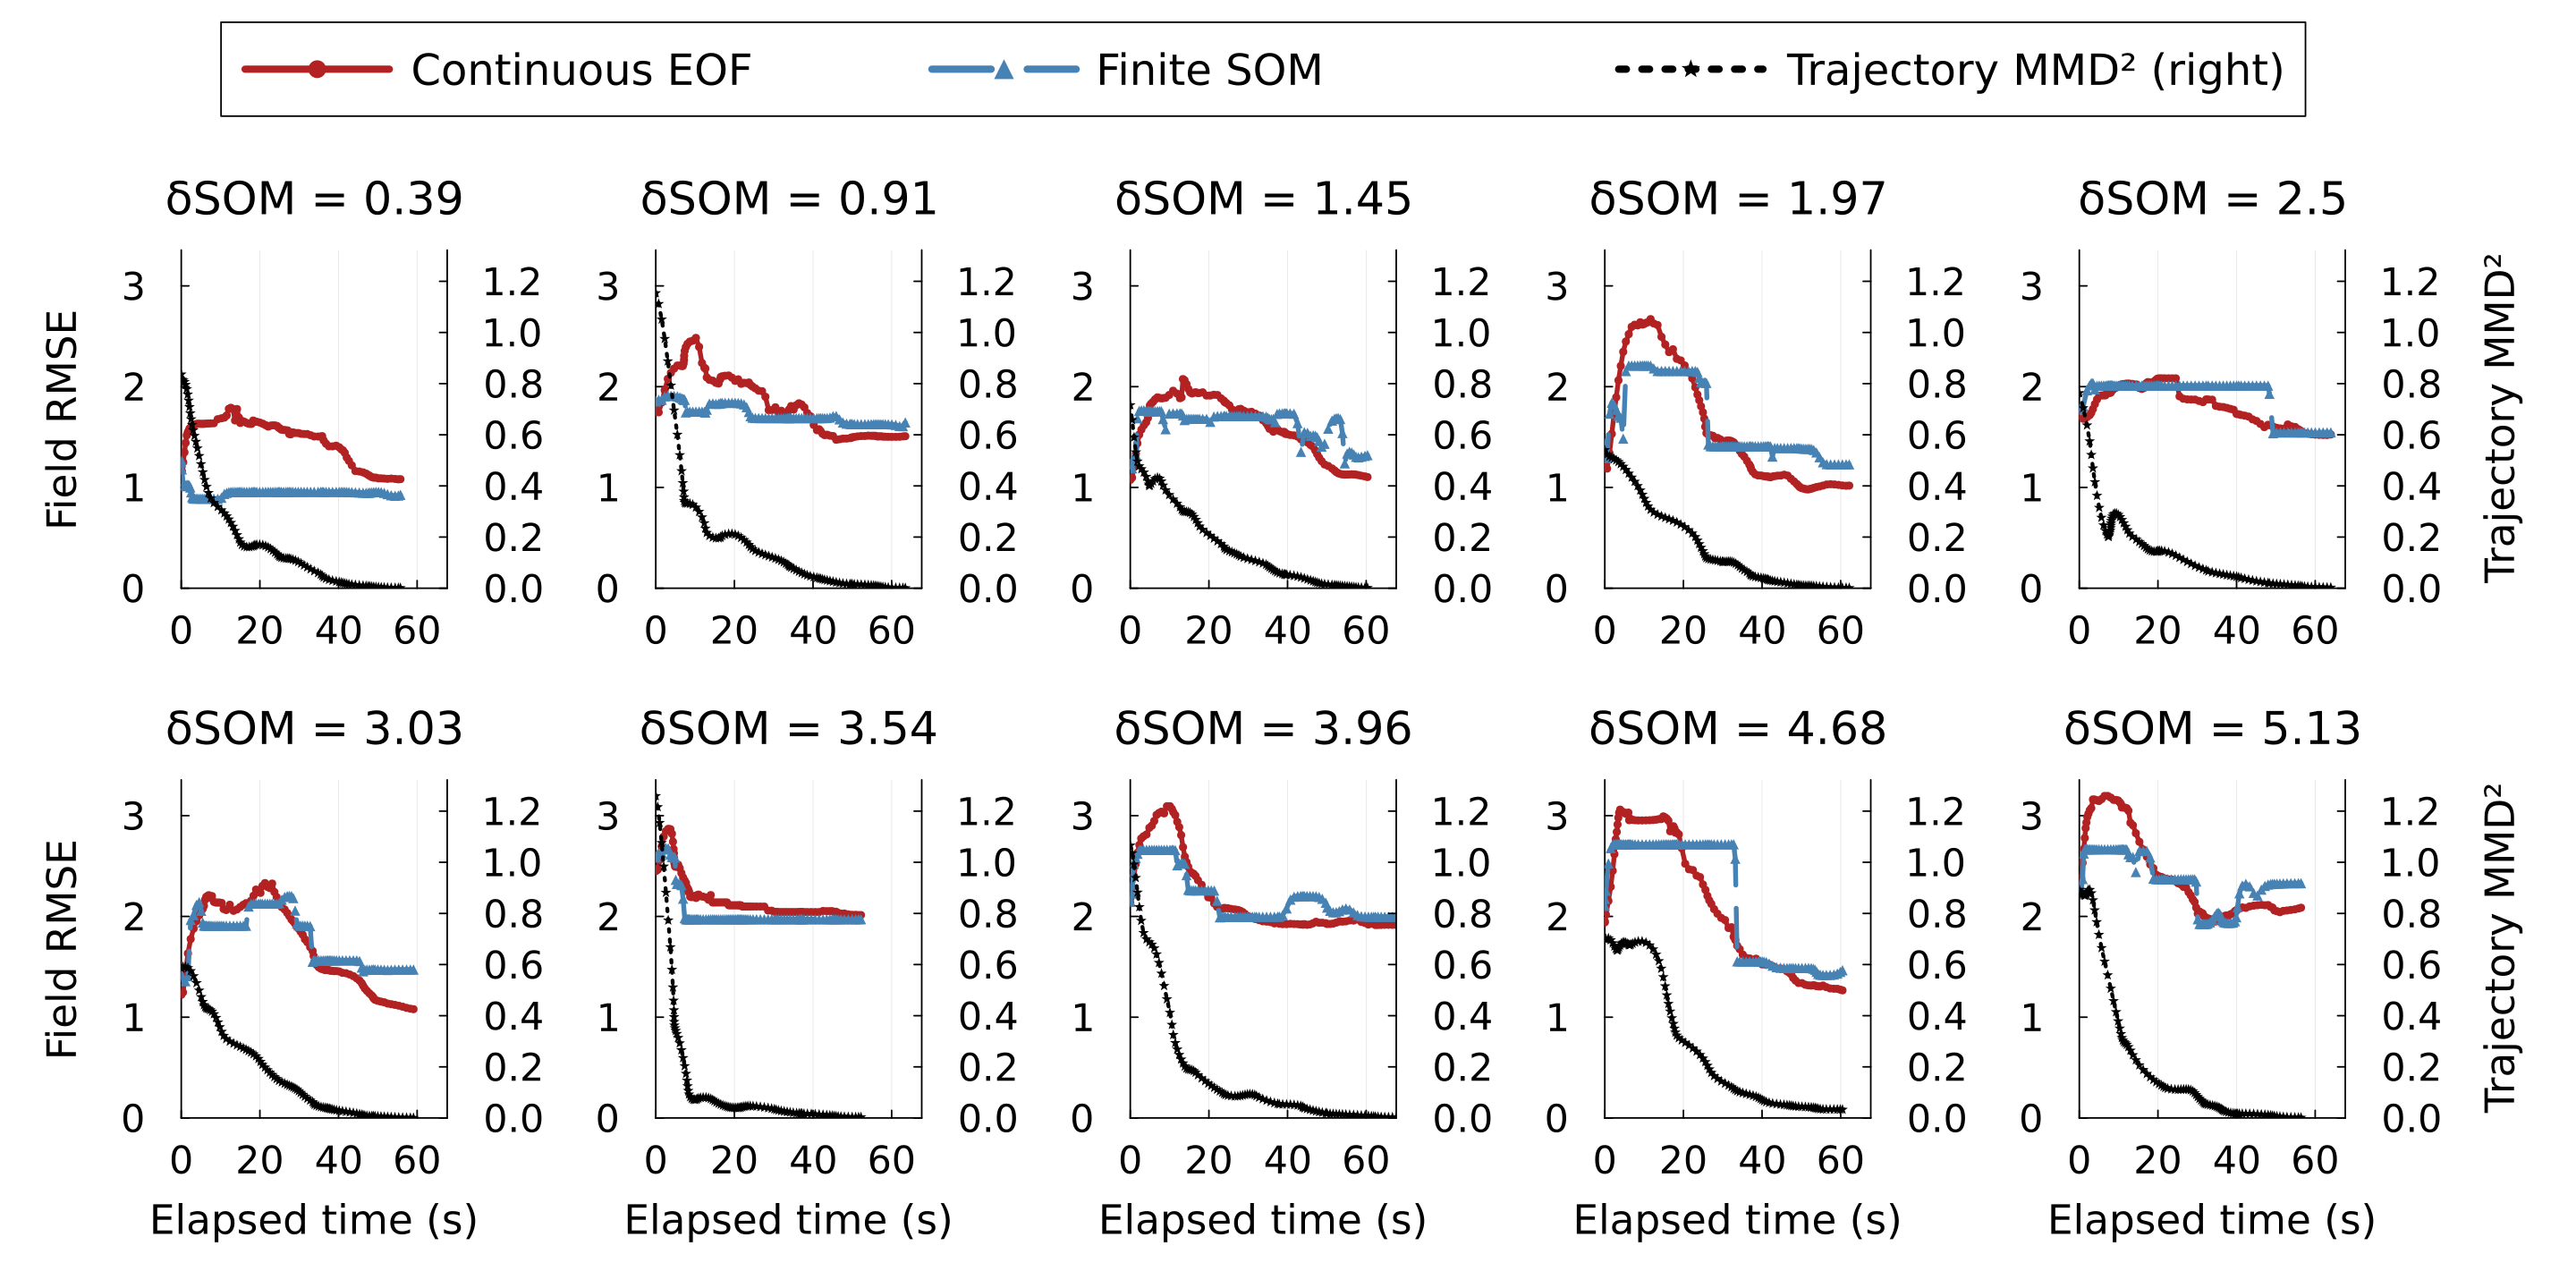
\includegraphics[width=\textwidth]{figs/all_recovery_histories.png}
  \caption{Finite SOM and continuous EOF reconstruction histories across increasing distance from the SOM region. Colored curves show field RMSE on the left axis; black stars show trajectory-to-generating-target MMD$^2$ on the right. Markers indicate observations at elapsed physical times, and panel labels give $\delta_{\mathrm{SOM}}$ in prior standard deviations. Finite reconstructions often settle early, whereas continuous recovery develops as the route covers the generating target. The generating target is used only for simulated evaluation.}
  \label{fig:recovery-histories}
\end{figure*}

The delay varies across fields: some EOF reconstructions improve rapidly after a sharp discrepancy decline, while others improve later in the route. The recurrent association is between declining discrepancy and better EOF reconstruction, providing an empirical basis for choosing when its greater capacity becomes useful.

\section{Discussion}

\subsection{Choosing between SOM and EOF Inference}

SOM inference is exact over its finite hypotheses, but approximate as a reconstruction of the observed agent's field. Its computational advantage comes from enumerating a small set of complete states; its accuracy depends on whether those states describe the belief being inferred. EOF inference relaxes this restriction by estimating continuous coefficients, at the cost of sampling a larger space of possible fields.

A short trajectory need not yet be ergodic with respect to the belief that generated it. EOF inference is particularly affected because it can construct alternative fields whose targets better match the visited locations. Longer observation histories reduce this ambiguity, allowing the continuous representation to improve on the finite approximation.

We therefore propose using the SOM reconstruction initially and treating a sharp decline in discrepancy as a signal to switch to EOF inference. The plotted discrepancy uses the known generating belief; an online rule must instead compare the trajectory with inferred targets. Because an incorrect field can also explain a short route, the reliability of that observable indicator must be evaluated before the proposed switch can be used operationally.

Fields farther from the SOM region place greater demands on continuous inference, but distance alone does not determine convergence time. A field with separated sampling regions may require many observations before all are represented in the trajectory. The histories consequently support a dependence on both departure from the prior representation and the spatial evidence accumulated during exploration.

\subsection{Coordination and Scientific Interpretation}

An AUV could use the inferred field to anticipate a teammate's sampling priorities and select complementary measurements. Differences between their models would identify regions where further observations are useful. Arrodes provides the missing model for this planning process; evaluating the resulting coordination is the next step.

For scientists aboard a support vessel, the reconstruction identifies the environmental assumptions behind a route. Repeated sampling around a predicted circulation feature becomes interpretable once that feature is visible in the inferred belief. Comparison with independent observations could then distinguish a scientifically useful response from a decision driven by an inaccurate onboard model.

\subsection{Scope and Extensions}

The simulated trials use static field beliefs, complete position traces, and a known curl-based sampling objective. They isolate inference of the environmental model from simultaneous uncertainty about goals or changes in the model during exploration. Extending the method to intermittent observations and evolving beliefs will require accounting for when a trajectory was generated under each estimate.

Our use of curl magnitude reflects the motivating interest in coastal circulation: it assigns sampling value to rotational structures in the flow data. The reconstruction is consequently a scalar field of this quantity, rather than a recovery of every velocity component or a direct estimate of vertical transport. Other scientific tasks can transform a field into sampling value differently; applying Arrodes then requires specifying that transformation and examining which aspects of the underlying field it preserves in behavior.

The SOM cannot reconstruct arbitrary unfamiliar fields, and the EOF model remains limited to combinations of its retained modes. The exploration objective also determines which field differences are observable: fields that induce the same sampling target cannot be distinguished by this behavioral model. Testing other objectives and informative planners would establish how broadly the discrepancy formulation applies beyond the ergodic trajectories considered here.

\section{Conclusion}

Arrodes extends belief inference to the environmental fields that guide exploratory sampling. SOM states provide a finite set of spatially resolved world hypotheses for exact Bayesian evaluation; EOF coefficients generalize these hypotheses to a continuous space that can represent beliefs outside the SOM's range. The simulated reconstructions show the resulting tradeoff: SOM inference gives an efficient early approximation, whereas EOF inference generally recovers the observed agent's belief more closely once enough of its trajectory has been observed. The relationship between recovery and declining ergodic discrepancy motivates switching between these approaches as evidence accumulates. This ability to reconstruct the model behind an exploration decision is a foundation for coordinating vehicles and explaining their behavior when their environmental knowledge cannot be shared directly.

\balance

\bibliographystyle{IEEEtran}
\bibliography{references}

\end{document}

% LocalWords:  discretizations centric
